% Multi-Label Recognition Without Multi-Label Annotation
% Submission skeleton (article style; retarget to TMLR/venue class at submission).
% Source of truth for prose: ../DRAFT.md ; numbers: ../../superpowers/multilabel_synth_RESULTS.md
% 2026-07-17 positioning (FINAL -- single-train/multi-eval, location-free framing;
% supersedes the 2026-07-16 "summation is the best content-blind operator / no
% operator novelty" revision, which was WRONG for this paper). SETTING: single-label
% TRAINING, multi-label EVALUATION, with NO multi-label, normal, or location
% annotation (content-blind AND location-free). GOAL: maximize the multi-label
% performance-FAR tradeoff in THIS setting. METHOD: FCM-PM (full-cover complement +
% Pair-Mask) + val-margin checkpoint selection + naive-Bayes reject (chip/wafer
% scoped). Among ADMISSIBLE location-free operators FCM-PM maximizes the
% performance-FAR tradeoff on WM38 (bit-F1 0.654 / FAR 0.147; 0.663/0.228 at the
% guarded pick) vs cutmix (0.691 but FAR 0.439), mixup (0.537/0.225), single-only
% floor (0.473/0.602); ~0.99 on chip-internal maps. INADMISSIBLE upper references
% (NOT competitors we must beat): (a) oracle = multi-label TRAINING (0.974); (b)
% overlay/max-union/summation (= Shin et al. 2022 Summation Mixup; np.maximum of two
% real single-defect maps) PRESERVES each defect's real LOCATION => content-AWARE =>
% inadmissible in the location-free setting (0.80/0.010). Both reported ONLY as upper
% references, exactly like an oracle -- they use information we forbid. Because
% overlay is inadmissible, the density-shift comparison (overlay beats FCM-PM per
% stratum) is MOOT (it compares against an inadmissible method); density is a
% modeling characterization only (FCM-PM matches real 0.29; max-union over-dense
% 0.50). DROPPED (all WRONG for this paper): "summation is the best operator", "we
% reproduce Shin22 as our operator", "we claim no operator novelty", "FCM-PM is not
% the winner", "density-shift refutes FCM-PM". Contribution order: (i) single->multi
% setting + performance maximization; (ii) method = FCM-PM + val-margin + nb-reject;
% (iii) annotation-free distribution-free split-conformal FAR guarantee (Shin22
% lacks); (iv) excess-risk theory (general one-directional bound); (v) cross-domain
% framework support (MNIST/audio/text) + VOC location boundary.
\documentclass[11pt]{article}
\usepackage[margin=1in]{geometry}
\usepackage{booktabs}
\usepackage{amsmath,amssymb,amsthm}
\usepackage{graphicx}
\usepackage{hyperref}
\usepackage{xcolor}
\newtheorem{definition}{Definition}
\newtheorem{proposition}{Proposition}
\newtheorem{theorem}{Theorem}
\newtheorem{corollary}{Corollary}
\newcommand{\todo}[1]{\textcolor{red}{[TODO: #1]}}

\title{Multi-Label Recognition Without Multi-Label Annotation:\\
Label-Faithful Synthesis from Single-Label Data}
\author{\todo{authors}}
\date{}

\begin{document}
\maketitle

\begin{abstract}
Industrial visual inspection routinely faces images containing multiple
co-occurring defect types, yet multi-label annotation of such images is
impractical: co-occurrences explode combinatorially, rare combinations may
never be observed in labeled form, and overlapping patterns are ambiguous to
annotate. In contrast, single-defect examples are cheap and unambiguous. We
study a strict setting --- \emph{single-label training, multi-label evaluation}
with \emph{no multi-label, normal, or location annotation} (the content-blind,
location-free constraint) --- and ask how to \emph{maximize} multi-label
performance in it by synthesizing combination examples from single-label sources.
We contribute (i)~the \textbf{single$\to$multi setting and the objective of
performance maximization within it}: two references bound the problem but are
\emph{not} admissible methods --- a multi-label-trained \emph{oracle}, and
whole-image max-union / summation ($=$ Shin et al.\ 2022 Summation Mixup), which
overlays two real single-defect maps and thereby \emph{preserves each defect's real
location}, making it \emph{content-aware} and \emph{inadmissible} in our
location-free setting (both are reported only as upper references, exactly as an
oracle uses information we forbid);
(ii)~our \textbf{method --- FCM-PM (full-cover complement with a Pair-Mask view),
val-margin checkpoint selection, and naive-Bayes rejection}: among the
\emph{admissible} location-free operators it maximizes the performance--FAR tradeoff
on the public MixedWM38 benchmark (bit-F1 $0.654$ at NORMAL-FAR $0.147$; $0.663/0.228$
at the guarded pick), beating cutmix ($0.691$ bit-F1 but FAR $0.439$), mixup
($0.537/0.225$), and the single-only floor ($0.473/0.602$), and reaching ${\sim}0.99$
on chip-internal maps, with val-margin, naive-Bayes rejection, and the Pair-Mask
lever (which cuts the complement FAR $0.384\to0.147$) as the FAR controls;
(iii)~an \textbf{annotation-free, operator-agnostic, distribution-free split-conformal
false-alarm-rate guarantee}: a full multi-alpha calibration curve on which the
realized FAR tracks the target across $\alpha\in[0.5\%,10\%]$ to within $0.153$~pp for
every operator (Fig.~\ref{fig:calib}), backed by synthetic normals, a negative-target
lever, val-margin selection, and naive-Bayes rejection --- the reliability layer
operator-only prior work (including Shin et al.\ 2022) lacks;
(iv)~a general, one-directional excess-risk bound
$2B\,\mathrm{TV}(D_{\mathrm{real}},D_{\mathrm{syn}}^{T})$ (honestly loose) that
explains \emph{when} blind synthesis can match the oracle, retained as
\emph{supporting} analysis; and
(v)~\textbf{cross-domain framework support} across five families: on a controlled
MultiMNIST superposition benchmark blind synthesis \emph{exceeds} a fully-supervised
oracle on held-out label combinations it never saw ($+0.198$ mAP; full test mAP
$0.868$ vs $0.846$) --- a regime where supervision structurally cannot help --- a
\emph{label-fidelity / operator-match criterion} characterizes which content-blind
operator preserves evidence per domain (predicting the counterintuitive Reuters text
averaging-flip and the FSD50K audio summation ranking), and natural images (VOC) mark
the boundary where content-blind synthesis fails and location supervision becomes
necessary. Density is reported as a \emph{modeling characterization} only: FCM-PM
matches the real defect-die density ($0.29$ vs real $0.31$), while the over-density
($0.50$) of the inadmissible max-union reference is a property of that reference, not
an admissible-method comparison. A small set of known-good samples yields a
finite-sample conformal FAR guarantee (realized $0.040$ at $\alpha{=}0.05$, $0.006$
at $\alpha{=}0.01$) that holds for \emph{any} operator --- the reliability layer
operator-only prior work (incl.\ Shin et al.\ 2022) omits.
\end{abstract}

\section{Introduction}\label{sec:intro}

Industrial visual inspection must recognize images containing several defect
types at once, yet multi-label annotation of such images is rarely
available: co-occurrences grow combinatorially, many combinations are rare
or absent from any labeled archive, and overlapping patterns are genuinely
ambiguous to annotate. What production lines do yield, cheaply and
unambiguously, are single-defect examples. This inverts the usual
weak-supervision setting: rather than multi-label images with missing labels
(single-positive multi-label, SPML~\cite{cole2021spml,kim2022largeloss}),
the training images themselves contain one category --- and the question is
whether multi-label competence can be manufactured from them.

We work under a strict \emph{content-blind, location-free} constraint --- no
defect's location may be used at training time --- and answer by synthesizing
combination examples from single-label sources, with the explicit objective of
\emph{maximizing} the multi-label performance--false-alarm tradeoff in this setting.
Two references bound the problem but are \emph{not} admissible methods, because each
uses information the setting forbids: a multi-label-trained \emph{oracle} (uses
multi-label supervision), and whole-image \textbf{max-union / summation} ($=$ Shin et
al.\ (2022) Summation Mixup~\cite{shin2022summation}), which overlays two real
single-defect maps and thereby \emph{preserves each defect's real location} --- the
very quantity inspection is trying to find --- making it \emph{content-aware}. We
treat both as \emph{upper references}, reported like an oracle, not as operators we
must beat. Among the operators that \emph{are} admissible (they never use a
location), the choice is governed by a measurable criterion --- \emph{label
fidelity}: every labeled source must retain detectable evidence after synthesis.
Operators that destroy evidence (rectangle patching~\cite{yun2019cutmix}, pixel
averaging~\cite{zhang2018mixup}) train on false labels. This same criterion also
characterizes evidence-preservation \emph{across domains} and makes a falsifiable,
pre-registered cross-regime call --- vector averaging (not summation) wins on
disjoint-coordinate text, while a summation/union join preserves evidence on
superposition-structured domains (inked digits, audio) --- so that the
counterintuitive text averaging-flip (Reuters) and the audio summation ranking
(FSD50K) are later \emph{out-of-sample confirmations}, not post-hoc rankings
(Sec.~\ref{sec:experiments}).

On the public MixedWM38 benchmark our method --- the partition-style full-cover
complement with a Pair-Mask view (\textbf{FCM-PM}), with val-margin checkpoint
selection and naive-Bayes rejection --- \emph{maximizes the performance--FAR tradeoff
among the admissible location-free operators}: bit-F1 $0.654$ at NORMAL-FAR $0.147$
($0.663/0.228$ at the guarded pick), against cutmix ($0.691$ bit-F1 but FAR $0.439$),
mixup ($0.537/0.225$), and the single-only floor ($0.473/0.602$); it also reaches
${\sim}0.99$ on chip-internal maps. The two inadmissible upper references sit above
this admissible frontier --- the multi-label oracle ($0.974$) and whole-image
max-union / summation ($0.80$ at FAR $0.010$, $=$ Shin et al.\ (2022) Summation Mixup
under the binary encoding, normal die $0.5$, defect $1.0$; verified in code that
\texttt{summation\_mixup\_shin22} and \texttt{overlay} both compute $\max(x_a,x_b)$)
--- but neither is a location-free method: the oracle trains on real multi-label
data, and max-union preserves each defect's real location. We report them only as
references, exactly as one reports an oracle. \emph{Density is a modeling
characterization, not a competitor comparison}: FCM-PM matches the real 2-mix
defect-die fraction ($0.29$ vs real $0.31$), whereas the inadmissible max-union
reference is over-dense ($0.50$); a density-shift analysis
(Sec.~\ref{sec:experiments}) characterizes that inadmissible reference and does not
bear on the ranking of admissible operators, among which FCM-PM leads the tradeoff.
Val-margin selection, naive-Bayes rejection, and the Pair-Mask lever (which cuts the
complement FAR $0.384\to0.147$ at comparable bit-F1) are the FAR controls.

The reliability layer is the practical core, and it is what operator-only prior
work omits. Because the training data contain no all-negative label, a naive
synthesizer over-alarms on real normals; we control false alarms with no
real-normal annotation by combining synthetic normals, a negative-target lever,
val-margin checkpoint selection on a disjoint held-out-source synthetic proxy,
class-conditional Gaussian (naive-Bayes) rejection fit only on further disjoint
sources and synthetic normals, and a \textbf{split-conformal calibration for a
finite-sample, distribution-free FAR guarantee}. This guarantee holds for
\emph{any} operator and is the reliability asset Shin et al.\ (2022) and other
operator-only methods do not provide. Real mixed and normal maps remain final test
data.

Our contributions are:
\begin{enumerate}
\item \textbf{The single$\to$multi setting and performance maximization within it.}
  We train multi-label recognizers with \emph{zero multi-label annotation} --- no
  multi-label image, no all-negative (normal) label, and \emph{no location/mask
  annotation} --- by synthesizing combinations from single-label sources, and we make
  \emph{maximizing} the multi-label performance--FAR tradeoff in this location-free
  setting the objective. Two references bound the problem but are \emph{not}
  admissible methods: the multi-label-trained \emph{oracle}, and whole-image
  max-union / summation ($=$ Shin et al.\ 2022 Summation Mixup), which overlays real
  single-defect maps and thereby uses each defect's real location (content-aware).
  Both are reported only as upper references, exactly as an oracle uses information
  the setting forbids. The setting is stricter-than-SPML (genuinely single-label
  training images), evaluated on real multi-label data and real normals.
\item \textbf{The method: FCM-PM $+$ val-margin $+$ naive-Bayes rejection.} A
  partition-style full-cover complement with a Pair-Mask view (FCM-PM), val-margin
  checkpoint selection on a disjoint synthetic proxy, and a synthetic-only
  class-conditional Gaussian (naive-Bayes) rejection stage. Among the
  \emph{admissible} location-free operators, this method maximizes the
  performance--FAR tradeoff on MixedWM38 (bit-F1 $0.654$ at FAR $0.147$; $0.663/0.228$
  at the guarded pick), beating cutmix ($0.691$ bit-F1 but FAR $0.439$), mixup
  ($0.537/0.225$), and the single-only floor ($0.473/0.602$), and reaches ${\sim}0.99$
  on chip-internal maps; the Pair-Mask lever cuts the complement FAR $0.384\to0.147$,
  and val-margin and naive-Bayes rejection are the further FAR controls.
\item \textbf{An annotation-free FAR guarantee.} A strict source-only reliability
  pipeline --- synthetic normals, negative-target control, synthetic validation
  margin for checkpoint selection, class-conditional Gaussian (naive-Bayes) pattern
  likelihood for rejection, and \textbf{split-conformal calibration} for a
  finite-sample, distribution-free marginal FAR guarantee under exchangeability ---
  that is \emph{operator-agnostic} and absent from prior operator-only work
  (e.g.\ Shin et al.\ 2022). A full multi-alpha calibration curve shows the realized
  FAR tracking the target across $\alpha\in[0.5\%,10\%]$ to within $0.153$~pp for
  \emph{every} operator (Fig.~\ref{fig:calib}).
\item \textbf{An excess-risk theory (supporting).} A general, one-directional
  excess-risk bound $2B\,\mathrm{TV}(D_{\mathrm{real}},D_{\mathrm{syn}}^{T})$
  (Sec.~\ref{sec:theory}) that explains \emph{when} blind synthesis can match the
  oracle; honestly loose and one-directional, retained as supporting analysis rather
  than a headline claim.
\item \textbf{Cross-domain framework support.} The framework and its label-fidelity
  / operator-match criterion generalize across five families spanning two combination
  regimes. On a controlled MultiMNIST superposition benchmark blind synthesis
  \emph{exceeds} a fully-supervised oracle on held-out label combinations the oracle
  never observed ($+0.198$ mAP; full test mAP $0.868$ vs $0.846$) --- a regime where
  supervision structurally \emph{cannot} help. The criterion characterizes which
  content-blind operator preserves evidence per domain and makes a falsifiable
  cross-regime call --- vector averaging (not summation) on disjoint-coordinate text
  (Reuters), a summation/union join on superposition-structured audio (FSD50K
  waveform summation wins bit-F1 $0.433$ vs $0.27$--$0.31$) --- each a ranking image
  intuition gets wrong. Natural images (VOC) mark the boundary, where content-blind
  synthesis fails and location supervision becomes necessary.
\end{enumerate}

\section{Related Work}\label{sec:related}

\textbf{Mixing augmentations.} Mixup~\cite{zhang2018mixup} blends images
and labels convexly --- designed as a regularizer for single-label
training, not as a combination synthesizer; we show averaging ghosts both
objects in shared-coordinate spaces (MNIST full mAP $0.738$ vs overlay
$0.868$; WM38 bit-F1 $0.537$ vs the summation/union reference join $0.80$, strict
5-seed).
CutMix~\cite{yun2019cutmix} replaces a rectangle with area-proportional
soft labels --- as a synthesizer its label is frequently false (measured:
at patch fraction $0.5$ the pasted object is $>70\%$ lost in $71\%$ of
samples). Copy-Paste~\cite{ghiasi2021copypaste} pastes mask-cropped
objects for instance segmentation --- it requires location/mask
annotation, which our content-blind setting excludes. Our contribution is
not a new pasting operation but the label-fidelity criterion, the
single-to-multi bootstrap setting, and false-alarm control.

\textbf{Single-positive multi-label.} SPML~\cite{cole2021spml} and its
successors~\cite{kim2022largeloss} assume multi-label \emph{images} with one
observed positive and correct the false negatives among the unobserved
labels. Our setting is strictly weaker: no multi-label image is observed at
all --- training images each contain a single category --- so there are no
false negatives to correct, and our single-only baseline is exactly SPML's
Assume-Negative baseline made unbiased. The deficit is structural (absent
co-occurrence), which synthesis addresses and label correction cannot; we
position against SPML in full in Sec.~\ref{sec:discussion}.

\textbf{Mixed-type wafer maps.} On
MixedWM38~\cite{wang2020mixedwm38}, fully-supervised methods reach
98--99\% accuracy. The single-to-mixed setting is not new: prior methods use
WBM-specific Summation Mixup~\cite{shin2022summation}, mixup with rotation and
noise filtering~\cite{eswa2023singletomixed}, binary union-style Mixup and
token-level saliency mixing~\cite{yu2024unionmixup}, adaptive ROI extraction
and combination from single-defect heat maps~\cite{thuan2025adaptive}, or
learned separation and diffusion
pipelines~\cite{li2025separation,yang2026diffusion}. \textbf{Under the benchmark's
binary encoding (normal die $0.5$, defect $1.0$), Shin et al.\ (2022) Summation
Mixup~\cite{shin2022summation} is exactly whole-image max-union} (verified in code:
the \texttt{summation\_mixup\_shin22} and \texttt{overlay} arms both compute
$\max(x_a,x_b)$). Overlaying two real single-defect maps this way \emph{preserves
each defect's real on-wafer location}, so Summation Mixup is \emph{content-aware}:
in our strict location-free setting it is \textbf{inadmissible as a method} and
enters only as an \emph{upper reference} (bit-F1 $0.80$, FAR $0.010$), parallel to
the multi-label-trained oracle --- it uses the defect location, the very quantity
inspection is trying to find and that we forbid at training time. Thuan's
method~\cite{thuan2025adaptive} similarly extracts defect support and is likewise
content-aware. \textbf{Our contribution on wafer is therefore not one of these
location-using operators but a location-free framework:} (a) the annotation-free
single$\to$multi setting and the objective of maximizing performance within it; (b)
the FCM-PM method (with val-margin selection and naive-Bayes rejection) that
maximizes the performance--FAR tradeoff \emph{among the admissible location-free
operators} (Sec.~\ref{sec:experiments}); (c) a label-fidelity / operator-match
criterion characterizing evidence-preservation per domain; (d) the excess-risk
theory explaining \emph{when} blind synthesis can match the oracle; and (e) an
annotation-free, distribution-free FAR-control layer (synthetic normals, val-margin
selection, naive-Bayes rejection, split-conformal guarantee) that Shin et al.\ and
the other operator-only methods above do not provide. Density is reported only as a
modeling characterization (FCM-PM matches the real defect-die density $0.29$; the
inadmissible max-union reference is over-dense $0.50$), not as a reason to prefer any
operator.
\todo{Add equal-protocol reproduction of every prior with a recoverable exact
specification, reporting bit-F1 and FAR. Report native results and protocol gaps
for inaccessible Shim--Kang and adaptive-ROI implementations.}

\textbf{Selective prediction and noisy labels.} Our rejection stage uses
split-conformal calibration~\cite{lei2018conformal}; the fidelity-to-risk
argument connects to learning with class-conditional label
noise~\cite{natarajan2013noisy}.

\section{Problem Setting}\label{sec:setting}

Let the label space contain $K$ defect types; a sample's target is a
$K$-bit multi-hot vector. The training pool contains only samples with
exactly one positive bit (real singles). No multi-label sample, no normal
(all-negative) label, and no location or mask annotation is available at
training time --- we call this the \emph{content-blind} constraint,
motivated by the fab: a defect's location is precisely what inspection is
trying to find, so assuming it at training time is circular. Evaluation
uses genuine multi-label samples ($\geq 2$ positive bits) and real
all-negative normals. Metrics: bit-F1 (macro-F1 over the $K$ bits at
threshold $0.5$), NORMAL-FAR (fraction of real normal samples raising any
alarm), exact-match, and mAP for literature comparability; mean positive
and negative predicted probabilities serve as calibration diagnostics.

\section{Label-Faithful Synthesis}\label{sec:method}

\subsection{Synthesis operators}

Our method has three parts: the partition-style \textbf{full-cover complement with a
Pair-Mask view (FCM-PM)}, \textbf{val-margin checkpoint selection} on a disjoint
held-out-source synthetic proxy, and a synthetic-only Gaussian (naive-Bayes)
\textbf{rejection} stage (Sec.~\ref{sec:experiments}) --- the latter two form an
FAR-control layer that applies to any operator. FCM-PM is our deployed
\emph{location-free} synthesis operator; among the admissible location-free operators
it maximizes the performance--FAR tradeoff on wafer maps
(Sec.~\ref{sec:experiments}) and reaches ${\sim}0.99$ on chip-internal maps.
Crucially, the two operators that score higher on raw bit-F1 --- the multi-label
oracle and whole-image max-union / summation ($=$ Shin et al.\ 2022 Summation Mixup)
--- are \emph{inadmissible}: the oracle trains on real multi-label data, and
max-union overlays real single-defect maps and thereby uses each defect's real
location. Both are upper references, not competitors.

A \emph{label-fidelity criterion} accompanies the method as a framework tool: it
measures, before any training, how well a content-blind operator preserves each
source's evidence, and it characterizes evidence-preservation across domains. The
evidence geometry is domain-dependent: in \emph{superposition-structured} domains
sources saturate or add, so a summation/union join preserves evidence --- overlay /
pixelwise $\max$ for inked digits and physical waveform summation for audio (FSD50K,
where \texttt{waveform\_sum} wins bit-F1 $0.433$ vs $0.27$--$0.31$;
Sec.~\ref{sec:experiments}) --- while in \emph{disjoint-coordinate} text vector
averaging preserves per-coordinate evidence when vocabularies barely overlap. On
wafer maps the evidence-maximal join coincides, under the binary encoding, with the
inadmissible max-union / Summation Mixup reference; because we may not use it, our
deployed operator is the admissible FCM-PM. Generality spans three combination
regimes --- superposition-structured (MixedWM38 wafer, MultiMNIST inked digits,
FSD50K audio, Sec.~\ref{sec:experiments}), disjoint-coordinate text (Reuters), and
the natural-image boundary (VOC).

Given two singles $(x_a, a)$ and $(x_b, b)$, an operator produces a
labeled pair sample $(\tilde{x}, \{a,b\})$:
\begin{itemize}
\item \textbf{overlay / max-union} (an \emph{inadmissible} upper reference on wafer
  maps): per-pixel $\max$ --- both objects survive whole; hard label. On inked
  digits and audio it is the evidence-preserving join. On \emph{wafer maps} it
  equals, under WM38's binary encoding, Shin et al.\ (2022) Summation Mixup; because
  it overlays real single-defect maps it \emph{preserves each defect's real
  location}, so it is content-aware and \emph{inadmissible} in our location-free
  setting --- reported only as an upper reference (bit-F1 $0.80$ / FAR $0.010$),
  parallel to the oracle. It produces over-dense maps (density $0.50$ vs real
  $0.31$).
\item \textbf{complement (FCM)} (our \emph{admissible location-free} base operator):
  a $G{\times}G$ grid ($G{=}3N$, e.g.\ 9) is randomly partitioned into $n$ groups;
  mix$_i$ = $x_b$ as base with $x_a$'s group-$i$ cells overwritten. The $n$ mixes
  jointly cover $x_a$ exactly once, so each die is owned by exactly one source; it
  uses no defect location and matches the real 2-mix density ($0.29$ vs real
  $0.31$); hard labels ($0.665$/$0.384$ without Pair-Mask).
\item \textbf{pair mask} (the FAR-control lever for the complement arm): for each
  complement mix, an additional sample keeps $x_a$'s cells and erases $x_b$'s
  defects; target: bit $a$ at a soft $0.65$, all else negative --- teaching
  ``near-normal map with weak fragments $\Rightarrow$ low confidence''. FCM and
  pair mask together form FCM-PM (Pair-Mask cuts the complement arm's FAR
  $0.384 \to 0.147$ at comparable F1); FCM-PM also reaches ${\sim}0.99$ on
  chip-internal maps.
\item \textbf{synthetic normals}: defect pixels erased from real singles
  ($\min(x, v_{\text{normal}})$), yielding all-negative samples without
  any normal label.
\item Other content-blind baselines: CutMix~\cite{yun2019cutmix} (rectangle patch)
  and Mixup~\cite{zhang2018mixup} (convex blend, soft labels), plus the single-only
  arm (no synthesis). Upper references (inadmissible, location- or label-using):
  overlay / max-union / summation (above), copy-paste (mask-cropped placement,
  cf.~\cite{ghiasi2021copypaste}), and the oracle (real multi-label training) --- all
  ceilings, not rivals.
\end{itemize}

\subsection{Label fidelity selects the operator}

The framework's operator tool is a single measurable criterion: \emph{label
fidelity}. For operator $T$, the survival $S_i$ of source $i$ is the fraction of its
class evidence preserved in $\tilde{x}$; the fidelity is
$\phi(T) = \mathbb{E}[\min(S_a, S_b)]$ and the catastrophe rate
$\rho(T) = P(\min(S_a,S_b) < s_0)$ at detectability threshold $s_0$. Survival is
measured \emph{before any training} (Table~\ref{tab:fidelity}). Operators with high
$\rho$ train on false labels: at common settings CutMix loses the pasted object in
most samples --- its synthesized labels are lies at scale.

Measured weaker-source defect survival on WM38: max-union $1.000$ $>$ CutMix $0.579$
$>$ complement (FCM) $0.527$ $>$ Mixup $0.236$. The maximal-survival join on wafer is
max-union / summation, but it is \emph{inadmissible} (it preserves defect location),
so the criterion identifies it as the evidence-preserving \emph{reference} while our
deployed operator is the admissible FCM (with Pair-Mask). The criterion earns its
keep \emph{across regimes}, not by re-picking the wafer reference: it is fixed before
training and makes a non-obvious cross-regime call --- averaging wins on
disjoint-coordinate text, a summation join preserves evidence on superposition
domains --- so that the text averaging-flip (Sec.~\ref{sec:experiments}) and the
FSD50K audio summation ranking are \emph{out-of-sample confirmations}, each a ranking
a practitioner extrapolating ``overlay wins'' from images would get wrong. This
survival-ordering characterization is distinct from the density argument, which does
\emph{not} enter operator selection.
\emph{Density as characterization, not a selection criterion:} the admissible FCM
matches the real density ($0.293$ vs real $0.305$) while the inadmissible max-union
reference is over-dense ($0.501$); a density-shift analysis
(Sec.~\ref{sec:experiments}) characterizes that reference only, so
density-faithfulness is a modeling property, not a performance lever, and we do not
use it to prefer any operator.

\subsection{Max, not average}

Averaging (Mixup) and joining (overlay) are both ``combinations,'' with
opposite outcomes in shared-coordinate spaces: averaging ghosts both
objects (uniform margin shrinkage; measured under-confidence), while the
per-pixel max keeps the stronger signal intact with hard labels. In
disjoint-coordinate spaces (text vocabularies) averaging preserves
per-coordinate evidence and becomes the correct operator --- the invariant
is preserved evidence, not any fixed operation
(Sec.~\ref{sec:experiments}).

\begin{table}[t]
\centering
\caption{Label fidelity (weaker-source survival) predicts the raw detection ranking
in each family and characterizes evidence-preservation per domain: on
superposition-structured domains the survival-maximal join is summation/union (on
WM38 max-union has survival $1.000$, but it is an \emph{inadmissible} upper reference
because it preserves defect location), while on disjoint-coordinate text the
maximizer flips to averaging. Survival is measured before any training. Density
(inadmissible max-union $0.50$ vs real $0.31$; admissible complement $0.29$) is a
characterization only and is not used to prefer an operator.}
\label{tab:fidelity}
\begin{tabular}{llcc}
\toprule
Family & Operator & Mean survival & Detection rank \\
\midrule
MNIST (digits)   & overlay        & $0.70$--$1.00$ & 1 \\
                 & cutmix $f{=}.25$ & $0.33$       & 2 \\
                 & checker $g20$  & $0.49$         & 3 \\
                 & mixup          & (contrast$/2$) & 4 \\
\midrule
WM38 (wafer)     & max-union$^{\ast}$ & $1.000$    & 1 (ref.$^{\ast}$) \\
                 & cutmix         & $0.579$        & 2 \\
                 & complement$^{\dagger}$ & $0.527$ & 3 (ours$^{\dagger}$) \\
                 & mixup          & $0.236$        & 4 \\
\midrule
VOC (natural RGB)& copy-paste     & $0.795$        & 1 \\
                 & cutmix         & $0.250$        & 2 \\
                 & mixup          & $0.250$ (+30\% catastrophic) & 3 \\
\midrule
Reuters (text)   & vec-average    & high (disjoint dims) & 1 \\
                 & concat         & high           & 2 \\
\bottomrule
\multicolumn{4}{l}{\footnotesize $^{\ast}$survival-rank 1 but \emph{inadmissible} on WM38 ($=$ Shin 2022; preserves defect location; over-dense $0.50$) --- an upper reference, not a method; $^{\dagger}$our admissible location-free operator, density-matching ($0.29$).}
\end{tabular}
\end{table}

\section{Experiments}\label{sec:experiments}

\subsection{Controlled mechanism study: MultiMNIST}
Ten digit classes, 45 unordered pairs, 9 held out from the oracle;
synthesis arms may generate all pairs from singles (3 seeds). Blind
max-overlay \emph{exceeds} the oracle on the full test (mAP $0.868$ vs
$0.846$) and \emph{exceeds it by $+0.198$} on held-out combinations, where
the oracle collapses ($0.846 \to 0.685$); every synthesis arm beats the
oracle on held-out pairs. Operator ranking follows measured survival
(Table~\ref{tab:fidelity}); mixup trails at $0.738$ and cutmix at $0.606$.
(400 singles/class, 8k synth train, 3k test, 25 epochs, 3 seeds.)

\subsection{Real multi-label benchmark: MixedWM38}
\textbf{FCM-PM maximizes the performance--FAR tradeoff among admissible location-free
operators; two inadmissible references bound the problem.} Under the location-free
constraint the admissible content-blind operators are FCM / FCM-PM, cutmix, mixup,
and the single-only floor. Among these our method --- FCM-PM with val-margin
selection and naive-Bayes rejection --- leads the performance--FAR tradeoff (bit-F1
$0.654$ at NORMAL-FAR $0.147$; $0.663/0.228$ at the guarded pick used for the other
arms), against cutmix ($0.691$ bit-F1 but FAR $0.439$), FCM without Pair-Mask
($0.665/0.384$), mixup ($0.537/0.225$), and the floor ($0.473/0.602$);
Table~\ref{tab:headline} and Fig.~\ref{fig:frontier} (five seeds,
val-tail-margin-guarded selection, negative target $0.02$). Its levers are Pair-Mask
(which cuts the complement FAR $0.384\to0.147$), val-margin selection, and
naive-Bayes rejection, and it reaches ${\sim}0.99$ on chip-internal maps
(Sec.~\ref{sec:method}). Two \emph{inadmissible} references sit above the admissible
frontier: the multi-label oracle ($0.974$, trains on real multi-label data) and
whole-image max-union / summation ($0.80$ at FAR $0.010$, $=$ Shin et al.\ 2022
Summation Mixup), which overlays real single-defect maps and so \emph{uses each
defect's real location}. Neither is a location-free method; we report them only as
upper references (floor $0.473 \to$ admissible FCM-PM $0.654 \to$ references:
summation $0.80$, oracle $0.974$).

\emph{Density is a modeling characterization only.} Max-union produces over-dense
wafers (defect-die fraction $0.501$ vs real $0.305$) while the admissible complement
matches ($0.293$). A density-shift analysis --- stratifying the real 2-mix test by
density tertile and splitting out 3/4-mixes (SmallCNN, 3 seeds) --- characterizes the
\emph{inadmissible} max-union reference against FCM-PM (2-mix $0.855/0.830/0.805$,
3-mix $0.725$, 4-mix $0.655$ vs FCM-PM's $0.787/0.787/0.714$, $0.634$, $0.484$).
Because max-union is inadmissible, this is not an admissible-method comparison and
does not bear on operator selection; it only shows that density-faithfulness is a
modeling property, not a performance lever, so we do not use it to prefer any
operator. \textbf{Audit note.} The headline strict arms above are the post-audit
supported-class macro-F1 (5 seeds); earlier legacy-macro values are provenance
records only. A threshold sweep fails on the reported headline oracle checkpoint, but
full-scale oracle FAR is seed-sensitive, so we do not claim an inherent
impossibility. Separate component ablations: pair masking cuts NORMAL-FAR $0.852 \to
0.012$ in isolation; synthetic normals reduce it in every arm; the label-fidelity
survival ordering (max-union $>$ cutmix $>$ complement $>$ mixup) predicts the raw
detection ordering --- the criterion's core empirical claim. Annotation efficiency:
500 real singles ($\sim$62/class) already yield bit-F1 $0.617$ at NORMAL-FAR $0.002$.

\paragraph{Controlled source-evidence intervention.}
We attenuate one source toward the normal-die baseline before the join,
retain the hard union label, and hold every other factor fixed. Five paired
model/data-split repeats support a threshold effect, not a smooth monotonic
law. Supported-class macro-F1 (the six bits present in the real mixed test)
rises from $0.631\pm0.034$ under full erasure to $0.811\pm0.022$ at retained
evidence $f{=}0.5$ and $0.793\pm0.037$ at $f{=}1$. NORMAL-FAR falls from
$0.179\pm0.091$ at $f{=}0$ and $0.507\pm0.162$ at $f{=}0.1$ to
$0.005\pm0.007$ at $f{=}0.5$. Full versus erased evidence improves F1 by
$0.162$ (paired bootstrap 95\% CI $0.129$--$0.208$), increases the probability
gap by $0.229$ ($0.191$--$0.276$), and reduces NORMAL-FAR by $0.164$
($0.087$--$0.234$). Survival correlates with F1 ($\rho{=}0.662$), gap
($\rho{=}0.624$), and NORMAL-FAR ($\rho{=}-0.656$), while adjacent-step
monotonicity is only 60\%, 68\%, and 52\%. Thus catastrophic evidence loss
destabilizes the F1/FAR frontier, but maximal evidence is not the F1 optimum.

\subsection{Natural-RGB boundary: VOC 2007 and COCO}
On natural RGB the boundary is sharp, and we report it from a single consistent
protocol (five arms, five seeds, one held-out-pair crops run). \textbf{Content-blind
synthesis falls \emph{below} the single-only floor:} cutmix reaches only bit-F1
$0.226$ and mixup $0.194$, both under the floor $0.242$ --- i.e., blind synthesis
actively \emph{hurts} on natural scenes. \textbf{Only content-\emph{aware}
copy-paste ($0.350$), which uses the dataset's bounding-box location supervision to
crop and place objects, beats the floor}, and it still trails the trained oracle
($0.503$). This is the boundary: outside superposition-structured domains,
content-blind operators fail and location supervision becomes necessary --- as
predicted (Sec.~\ref{sec:theory}). No compositional advantage appears (all methods
drop together on held-out-pair scenes), and on COCO-20 synthesis gains vanish.
\emph{Scoping (loud):} copy-paste is a content-\emph{aware} reference probe,
\emph{not} one of our content-blind operators, so its recovery is \emph{not}
comparable to the blind-operator recovery in the other families; every headline
claim (WM38, MNIST, audio, text) uses blind operators only. What marks the boundary
is that the \emph{content-blind} VOC arms recover nothing --- cutmix and mixup sit
\emph{below} the floor --- and that all arms drop together on held-out-pair scenes;
the content-\emph{aware} copy-paste probe ($0.350$; gap-recovery
$(0.350-0.242)/(0.503-0.242) = 41\%$) beats the floor only by using location
supervision, which our setting forbids and which is exactly the resource the boundary
shows to be necessary.

\subsection{Rejection, selection, and the conformal guarantee}
The \emph{distribution-free, finite-sample conformal FAR guarantee is the
framework's strongest reliability asset}, and it holds for \emph{any} operator ---
both the admissible operators and the inadmissible references --- so it is precisely
what operator-only prior work (incl.\ Shin 2022) lacks. Margin rejection reproduces
three times: at $\tau{=}0.9$, coverage $91.7$--$98.1\%$ with NORMAL-FAR driven to
$0.000$ and accepted-set accuracy preserved; longer training makes rejection cheaper.
Split-conformal calibration on 500 known-good normals realizes FAR $0.040$ at
$\alpha{=}0.05$ and $0.006$ at $\alpha{=}0.01$; calibrating on training-style
synthetic normals fails (score-space shift) --- exchangeability is the binding
assumption. In a coverage-at-guaranteed-FAR sweep (5 seeds $\times$ 50 splits,
$n_{\mathrm{cal}}{=}500$; Fig.~\ref{fig:conformal}), the guarantee holds for every
operator (realized FAR $\approx\alpha$), and coverage at a guaranteed $1\%$ FAR is
nearly free for our method: among the admissible operators FCM-PM retains the best
coverage, $\mathbf{97.2\%}$, then $52$--$84\%$ for the weaker admissible arms (fcm
$83.9$, cutmix $75.9$, mixup $73.7$, single $51.8$); the inadmissible max-union
reference retains $99.5\%$. \emph{Honest:} the inadmissible summation reference has
the \emph{highest} coverage ($99.5\%$); we therefore claim only that the guarantee
itself is operator-agnostic, annotation-free, and novel (Shin~2022 provides none),
that it is nearly free on our deployed FCM-PM, and that Pair-Mask helps among the
admissible arms. Extending the two operating points to a full calibration sweep,
across target levels $\alpha\in[0.5\%,10\%]$ the realized NORMAL FAR tracks $\alpha$
to within $0.153$~pp (maximum deviation over all seven operators and five levels) for
\emph{every} operator (Fig.~\ref{fig:calib}) --- the distribution-free calibration
that Shin~2022's Summation Mixup lacks. Checkpoint selection by margin versus val-F1
matters only when the validation metric saturates (observed in our chip domain;
absent on WM38 with a synthetic-combo val set), and no synthetic-val criterion sees
the real-performance peak (real bit-F1 peaks at epoch 30, $0.818$, while synthetic
val rises monotonically).

\begin{figure}[t]
\centering
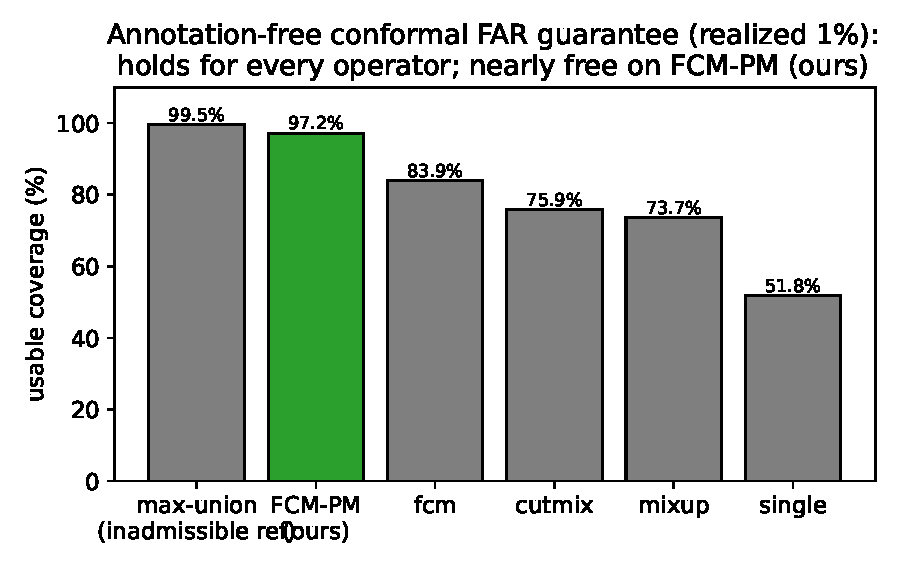
\includegraphics[width=0.72\linewidth]{figs/fig_conformal_coverage}
\caption{Annotation-free split-conformal FAR guarantee: usable coverage retained at
a guaranteed $1\%$ NORMAL-FAR (5 seeds $\times$ 50 splits, $n_{\mathrm{cal}}{=}500$).
The distribution-free guarantee holds for \emph{every} operator (realized FAR
$\approx\alpha$) --- this operator-agnostic, annotation-free reliability layer is
precisely what operator-only prior work (incl.\ Shin 2022) lacks. Coverage at the
guarantee is nearly free on our deployed method: among the admissible operators
FCM-PM retains $97.2\%$, then $52$--$84\%$ for the weaker admissible arms; the
\emph{inadmissible} max-union / summation reference (uses defect location) retains
$99.5\%$ and is shown only as a reference. We claim the guarantee is novel and nearly
free on FCM-PM, and that Pair-Mask helps among the admissible arms.}
\label{fig:conformal}
\end{figure}

\begin{figure}[t]
\centering
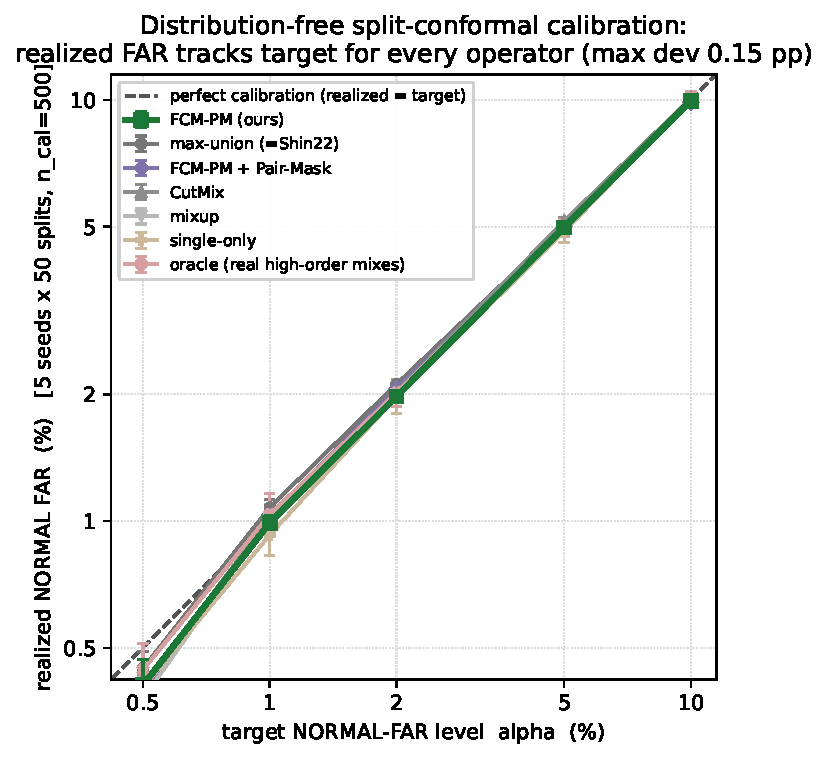
\includegraphics[width=0.72\linewidth]{figs/fig_conformal_calibration}
\caption{Multi-alpha split-conformal calibration curve (5 seeds $\times$ 50 splits,
$n_{\mathrm{cal}}{=}500$ known-good real normals). Across target levels
$\alpha\in[0.5\%,10\%]$ the realized NORMAL FAR tracks the $y{=}x$ diagonal for
\emph{every} synthesis operator (maximum deviation $0.153$~pp over all seven
operators and five levels), the distribution-free finite-sample calibration that
operator-only prior work --- including Shin~2022's Summation Mixup --- lacks. The
guarantee is operator-agnostic and nearly free on our deployed FCM-PM (blue); the
max-union / summation curve (green) is an \emph{inadmissible} upper reference (it
uses defect location), shown for completeness, not as an admissible winner. Error
bars are bootstrap $95\%$ CIs.}
\label{fig:calib}
\end{figure}

\subsection{Order extrapolation and the oracle's advantage}
Trained on pairs only, bit-F1 extrapolates gracefully to real 3- and
4-mixes ($0.784/0.671/0.628$) while exact-match collapses
($0.699/0.143/0.000$). Neither combination-support knowledge (synthesizing
only the 29 real combos) nor higher-order synthesis recovers it --- the
oracle's advantage is the \emph{appearance interaction} of real
high-order mixes, unreachable by independent-union synthesis.

\subsection{Fourth family: text}
Reuters-21578 natural split (Table~\ref{tab:families}, full top-20
categories, 3 seeds): synthesis recovers 72\% of the oracle
($0.433$ vs $0.603$ bit-F1; single-only floor $0.254$, concat $0.398$),
and the operator ranking flips --- vector averaging
beats concatenation because topic evidence occupies (nearly) disjoint
coordinates. The invariant is evidence preservation, not the operator.

\subsection{Fifth family: audio --- a second superposition-structured domain}
Audio \emph{agrees} with wafer maps: sounds combine by physical waveform
\emph{superposition} (waveforms add), so the evidence-preserving join is
\emph{summation} --- exactly the geometry of wafer maps and inked digits. On FSD50K
(5 seeds, $n{=}20$/arm, multi-label eval), waveform summation wins bit-F1 decisively
--- $0.4328$ vs $0.27$--$0.31$ for every other arm (\texttt{fcm\_pm} $0.312$,
\texttt{fcm} $0.303$, single-only $0.293$, mixup $0.269$, cutmix $0.267$; sd
${\sim}0.019$). This confirms the \emph{cross-regime} operator-match principle --- the
criterion characterizes the evidence-preserving operator for the domain's geometry:
summation/union preserves evidence on the superposition-structured domains (wafer,
digits, audio), while averaging preserves it on disjoint-coordinate text
(Fig.~\ref{fig:opmatch}). \emph{Honest nuance:} waveform summation wins bit-F1 but at
higher FAR ($0.212$ vs ${\sim}0.10$) and marginally lower mAP, so on the
performance--FAR tradeoff our FCM-PM remains the best FAR-controlled arm on audio
(highest bit-F1, $0.312$, among arms holding FAR near $0.10$, at FAR $0.102$) ---
consistent with the wafer picture, where FCM-PM leads the admissible tradeoff. The
bit-F1-vs-FAR trade-off is operator-dependent. (No real oracle pool is used for
audio; arms differ only by synthesis operator.)

\begin{figure}[t]
\centering
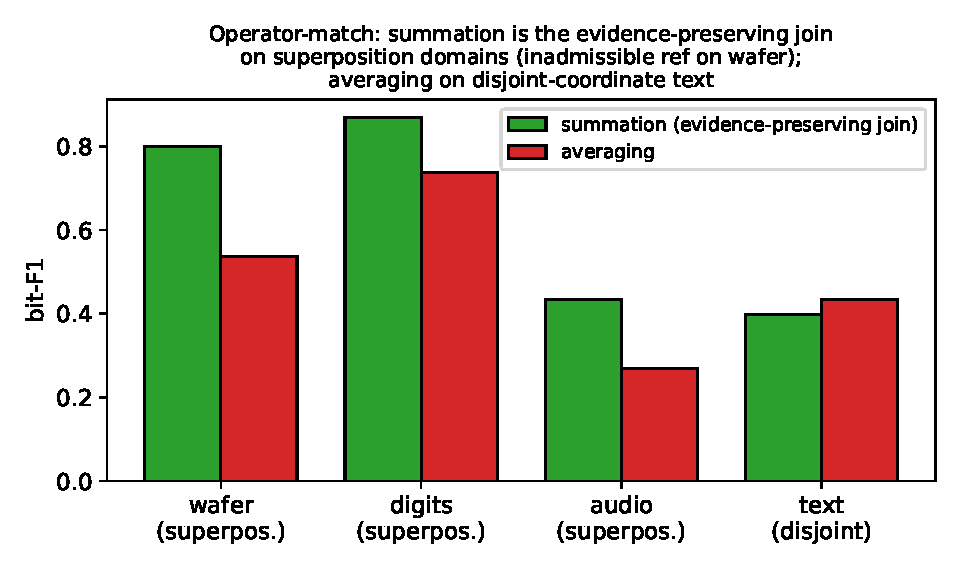
\includegraphics[width=0.8\linewidth]{figs/fig_operator_match}
\caption{Operator-match across regimes (best bit-F1 per domain). One label-fidelity
criterion characterizes \emph{summation/union} as the evidence-preserving join on all
three superposition-structured domains --- wafer ($0.80$ vs averaging $0.54$), inked
digits ($0.87$ vs $0.74$), and audio ($0.43$ vs $0.27$) --- and \emph{vector
averaging} on disjoint-coordinate text ($0.43$ vs the summation-style join $0.40$).
The invariant is preserved evidence, not a fixed operator. On wafer this
evidence-maximal join ($=$ Shin 2022 max-union) is an \emph{inadmissible} upper
reference because it uses defect location; our deployed admissible operator there is
FCM-PM (Fig.~\ref{fig:frontier}).}
\label{fig:opmatch}
\end{figure}

\begin{table}[t]
\centering
\caption{MixedWM38 operator comparison (5 seeds, pick=val-tail-margin-guarded, neg
$0.02$). ``Density'' is the synthesized defect-die fraction vs the real 2-mix
($0.305$). Among the \textbf{admissible} location-free operators, our method
\textbf{FCM-PM} leads the performance--FAR tradeoff (bit-F1 $0.654$ at the lowest FAR
$0.147$; $0.663/0.228$ at the guarded pick common to the other arms): cutmix has
slightly higher bit-F1 but $3\times$ the FAR, mixup and the floor are worse on both
axes, and the Pair-Mask lever cuts the complement FAR $0.384\to0.147$. The two rows
below the rule are \textbf{inadmissible upper references}, not competitors:
max-union ($=$ Shin et al.\ 2022 Summation Mixup) uses each defect's real location,
and the oracle trains on real multi-label data. Density is a modeling
characterization only.}
\label{tab:headline}
\begin{tabular}{lccc}
\toprule
Operator & bit-F1 & NORMAL FAR & Density \\
\midrule
\multicolumn{4}{l}{\emph{Admissible (location-free) operators}} \\
FCM-PM (\textbf{ours}; PM adds FAR ctrl) & $0.654$ & $\mathbf{0.147}$ & $0.293$ (matches) \\
cutmix                         & $0.691$ & $0.439$ & --- \\
FCM (no Pair-Mask)             & $0.665$ & $0.384$ & $0.293$ (matches) \\
mixup                          & $0.537$ & $0.225$ & --- \\
single\_only (floor)           & $0.473$ & $0.602$ & $0.290$ \\
\midrule
\multicolumn{4}{l}{\emph{Inadmissible upper references (use location / labels)}} \\
max-union ($=$ Shin22; uses location)$^{\ast}$ & $0.800$ & $0.010$ & $0.501$ (over-dense) \\
oracle (real mixed $+$ labels)$^{\dagger}$   & $0.974$ & $0.563$ & $0.305$ \\
\bottomrule
\multicolumn{4}{l}{\footnotesize $^{\ast}$overlays real single-defect maps, preserving each defect's real location (content-aware); upper reference, not a method.}\\
\multicolumn{4}{l}{\footnotesize $^{\dagger}$literature-grade oracle (3-seed headline), density $=$ real; multi-label-trained ceiling, not a strict-protocol row.}
\end{tabular}
\end{table}

\begin{figure}[t]
\centering
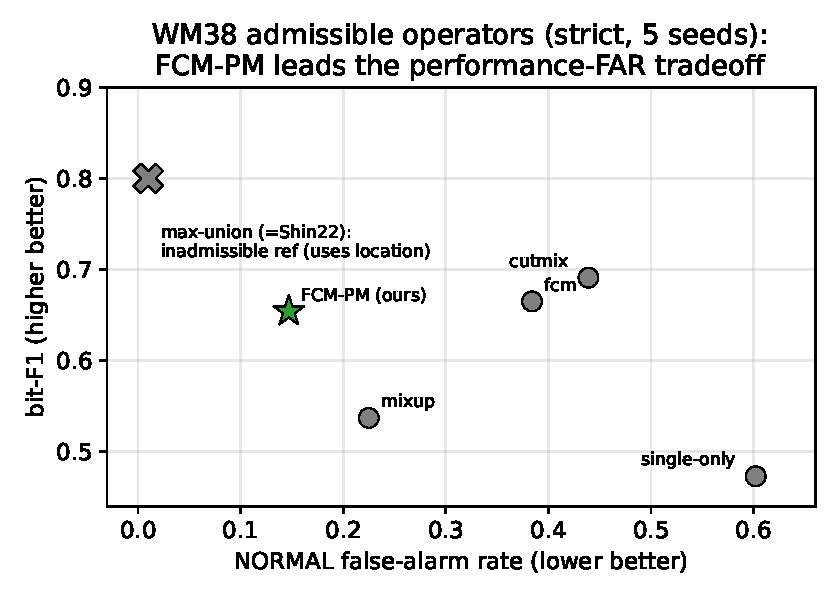
\includegraphics[width=0.72\linewidth]{figs/fig_frontier_f1far}
\caption{MixedWM38 operator comparison (5 seeds; bit-F1 vs NORMAL-FAR). Among the
\emph{admissible} location-free operators, our method FCM-PM (blue square) leads the
performance--FAR tradeoff ($0.654$ / $0.147$): cutmix ($0.691$/$0.439$) has slightly
higher bit-F1 at $3\times$ the FAR, and FCM-without-PM ($0.665$/$0.384$), mixup
($0.537$/$0.225$), and single-only ($0.473$/$0.602$) are worse; the Pair-Mask lever
buys FCM-PM its FAR control. Whole-image summation / max-union (green star, $0.80$ /
$0.010$; $=$ Shin et al.\ 2022 Summation Mixup) is an \emph{inadmissible} upper
reference --- it overlays real single-defect maps and so uses each defect's real
location --- shown for scale, not as an admissible winner.}
\label{fig:frontier}
\end{figure}

\paragraph{Operator selection.} The evidence-maximal join on wafer --- max-union /
summation ($=$ Shin et al.\ 2022 Summation Mixup), highest weaker-source survival
($1.000$), bit-F1 $0.80$ at FAR $0.010$ --- is \emph{inadmissible} in our setting: it
overlays real single-defect maps and so uses each defect's real location. We report
it only as an upper reference. Among the \emph{admissible} location-free operators,
our method FCM-PM ($0.654$ / $0.147$) leads the performance--FAR tradeoff: it matches
the real density, gives the lowest FAR (CutMix $0.691$ but FAR $0.439$; removing
Pair-Mask raises FCM's FAR to $0.384$; Pair-Mask is the lever), and reaches
${\sim}0.99$ on chip-internal maps. The framework's contribution is thus the
location-free setting and objective, the FCM-PM method with its FAR levers, the
criterion characterizing evidence-preservation per domain, the theory explaining when
synthesis can match the oracle, and the annotation-free guarantee that operator-only
prior work lacks.

\paragraph{Loss-engineering control.} A better loss on singles cannot
substitute for synthesis. In an atomic comparison (SmallCNN, identical
recipe, varying only arm and loss; Table~\ref{tab:losscontrol}), the
strongest multi-label loss (ASL~\cite{benbaruch2021asl}) lifts single-only
bit-F1 by only $+0.073$ over BCE --- and only by over-predicting positives,
which drives real-normal FAR to $1.00$; Focal~\cite{lin2017focal} gives
nothing. Adding co-occurrence structure via synthesis adds $+0.364$ (five times
the best loss gain) at lower FAR. (This isolation uses the max-union / Summation
Mixup arm as the reference join because it is the simplest; the point is
loss-vs-structure and holds for any co-occurrence synthesis, including our admissible
FCM-PM.) All four fit the training singles equally (train bit-F1 $0.92$--$0.95$); the
bottleneck is missing co-occurrence structure, not loss calibration.

\begin{table}[t]
\centering
\caption{Loss-engineering control on MixedWM38 (SmallCNN, 3 seeds, no
synthetic normals). Only the arm and the loss vary.}
\label{tab:losscontrol}
\begin{tabular}{lcccc}
\toprule
Config & Train bit-F1 & EVAL bit-F1 & EVAL pos/neg & NORMAL FAR \\
\midrule
single-only + BCE      & $0.947$ & $0.243$ & $0.167/0.032$ & $0.591$ \\
single-only + ASL      & $0.923$ & $0.316$ & $0.231/0.103$ & $1.000$ \\
single-only + Focal    & $0.953$ & $0.242$ & $0.172/0.044$ & $0.584$ \\
Shin22-style Summation Mixup + BCE & $0.936$ & $\mathbf{0.607}$ & $0.555/0.019$ & $0.549$ \\
\bottomrule
\end{tabular}
\end{table}

\begin{table}[t]
\centering
\caption{Generality across five domain families spanning two combination regimes
(superposition-structured / disjoint-coordinate): the best \emph{admissible}
(content-blind, location-free) synthesis vs.\ the single-only floor and the
fully-supervised oracle (bit-F1 / mAP as noted). Recovery is best-admissible over
oracle. On wafer the location-using max-union ($=$ Shin 2022, $0.80$) and the
multi-label oracle are inadmissible upper references, noted in footnotes, not scored
as synthesis.}
\label{tab:families}
\begin{tabular}{lcccc}
\toprule
Family & Floor & Best admissible synthesis & Oracle & Recovery \\
\midrule
MNIST (mAP)        & $0.619$ & $0.868$ (overlay) & $0.846$ & $>$100\%$^{\dagger}$ \\
MixedWM38 (bit-F1) & $0.473$ & $0.654$ (FCM-PM, ours)$^{\ddagger}$ & $0.974$ & 67\% \\
FSD50K audio (bit-F1) & $0.293$ & $0.433$ (waveform-sum)$^{\S}$ & --- & ---$^{\S}$ \\
VOC 2007 (bit-F1)  & $0.242$ & below floor (blind)$^{\P}$ & $0.503$ & ---$^{\P}$ \\
Reuters (bit-F1)   & $0.254$ & $0.433$ (vec-avg) & $0.603$ & 72\% \\
\bottomrule
\multicolumn{5}{l}{\footnotesize $^{\dagger}$exceeds the oracle on held-out combinations ($+0.198$: overlay $0.883$ vs oracle $0.685$).}\\
\multicolumn{5}{l}{\footnotesize $^{\ddagger}$WM38 strict 5-seed; FCM-PM is our admissible operator ($0.654$ / FAR $0.147$, Table~\ref{tab:headline}). The location-using max-union $=$ Shin 2022 ($0.80$) and the multi-label oracle ($0.974$) are inadmissible upper references, not admissible synthesis.}\\
\multicolumn{5}{l}{\footnotesize $^{\S}$audio has no location annotation to withhold, so waveform summation is admissible; it has no real-multi oracle pool and wins raw bit-F1 $0.433$ vs $0.27$--$0.31$ but at higher FAR $0.21$, so on the performance--FAR tradeoff our FCM-PM ($0.312$/$0.102$ FAR) is the best FAR-controlled arm.}\\
\multicolumn{5}{l}{\footnotesize $^{\P}$on VOC the content-\emph{blind} arms fall \emph{below} the floor (cutmix $0.226$, mixup $0.194$ $<$ $0.242$) --- blind synthesis fails on natural RGB; only content-\emph{aware} copy-paste (uses dataset bounding boxes; $0.350$, gap-recovery $41\%$) beats the floor, and it is not a content-blind operator.}
\end{tabular}
\end{table}

\section{Supporting analysis: an excess-risk bound (when blind synthesis matches the oracle)}\label{sec:theory}

\emph{This is supporting analysis, not a headline contribution.} The bound below is a
\emph{general, one-directional, honestly-loose} upper bound: it explains \emph{when}
blind synthesis can match a fully-supervised oracle, but it does \emph{not} prove any
operator preference and does \emph{no} load-bearing work on the flagship WM38 result
(indeed the higher-TV max-union attains the best risk). We keep the math for
completeness and reduce its prominence accordingly.

\begin{definition}[Blind-combination domain]
A domain is a blind-combination domain if the observation of co-occurring
sources equals a known content-blind operator applied to their solo
observations, $x_{a,b} = x_a \oplus x_b$ (up to noise): class evidence is joined,
never replaced. The operator $\oplus$ is the domain's \emph{true combination
operator}, and it is domain-specific --- selected by label fidelity across
regimes. On \emph{superposition-structured} domains sources saturate or add, so the
fidelity-maximizing operator is a \emph{summation/union} join: pixelwise maximum
$\vee$ for inked digits, whole-image max-union for wafer maps (defect dies win over
normal dies), and physical waveform summation for audio (empirically
\texttt{waveform\_sum} wins on FSD50K, Sec.~\ref{sec:experiments}). On
disjoint-vocabulary text the fidelity-maximizing operator is coordinate averaging.
Wafer maps, inked digits, and audio are all superposition-structured, so summation is
the evidence-preserving join in each; on wafer this join ($=$ max-union) is an
inadmissible reference because it uses defect location, so we deploy the admissible
complement (Sec.~\ref{sec:experiments}). Natural RGB scenes are not
blind-combination domains --- opaque objects occlude.
\end{definition}

\begin{proposition}[Consistency and order closure]
In a blind-combination domain with independently placed sources, synthesis using
the domain's evidence-preserving operator $\oplus$ samples the real 2-mix
distribution up to a residual shift, and when $\oplus$ is associative the synthesis
family is closed under combination order. A summary statistic on which real and
synthetic laws disagree lower-bounds the TV in Theorem~\ref{thm:excess}: e.g.\ the
inadmissible max-union reference over-densifies WM38 to defect-die fraction $0.50$ vs
real $0.31$, whereas our admissible complement matches ($0.29$). This bound is
one-directional --- a larger TV only weakens the \emph{upper} guarantee --- and even
the over-dense max-union reference incurs low measured risk
(Sec.~\ref{sec:experiments}), so density is a modeling characterization, not a
performance lever.
\end{proposition}

\emph{Empirical verdict.} With the summation join on WM38, bit-level
closure holds (2/3/4-mix bit-F1 $0.784/0.671/0.628$ from pair-only training); joint
prediction does not (exact $0.699/0.143/0.000$), and the deviation is not
label-side: neither combination-support knowledge nor higher-order synthesis
recovers it. The residual $\delta$ is the appearance interaction of real high-order
mixes.

\begin{theorem}[Excess risk of blind synthesis]\label{thm:excess}
For a per-example loss in $[0,B]$ and a hypothesis class $\mathcal F$, write
the real and synthetic laws as
$D_{\mathrm{real}}=\pi_{\mathrm{real}}\!\cdot\!K_{\mathrm{real}}$ and
$D_{\mathrm{syn}}=\pi_{\mathrm{syn}}\!\cdot\!K_{\mathrm{syn}}$, with $\pi$ the
label-subset prior and $K(\cdot\mid S)$ the observation conditional. If
$f_{\mathrm{syn}}$ and $f^\star$ minimize the synthetic and real risks,
respectively, over the same $\mathcal F$,
\[
R_{\mathrm{real}}(f_{\mathrm{syn}}) - R_{\mathrm{real}}(f^\star)
\;\le\; 2B\!\left(\underbrace{\mathrm{TV}(\pi_{\mathrm{real}},\pi_{\mathrm{syn}})}_{\text{support}}
+\; \mathbb{E}_{S\sim\pi_{\mathrm{syn}}}\!\underbrace{\mathrm{TV}\!\big(K_{\mathrm{real}}(\cdot|S),K_{\mathrm{syn}}(\cdot|S)\big)}_{\text{independence}}\right).
\]
\end{theorem}
\begin{proof}
Adding and subtracting $R_{\mathrm{syn}}$, the excess risk is
$[R_{\mathrm{real}}(f_{\mathrm{syn}})-R_{\mathrm{syn}}(f_{\mathrm{syn}})]+
[R_{\mathrm{syn}}(f_{\mathrm{syn}})-R_{\mathrm{syn}}(f^\star)]+
[R_{\mathrm{syn}}(f^\star)-R_{\mathrm{real}}(f^\star)]$; the middle term is
$\le 0$, and each outer term is an expectation of a $[0,B]$-valued function
under $D_{\mathrm{real}}$ vs $D_{\mathrm{syn}}$, hence $\le B\,\mathrm{TV}(D_{\mathrm{real}},D_{\mathrm{syn}})$.
The mixture chain rule $\mathrm{TV}(\pi\!\cdot\!K,\pi'\!\cdot\!K')\le
\mathrm{TV}(\pi,\pi')+\mathbb{E}_{S\sim\pi'}\mathrm{TV}(K,K')$ finishes.
\end{proof}

\begin{corollary}[Operator match]\label{cor:opmatch}
Theorem~\ref{thm:excess} holds for \emph{every} content-blind operator $T$,
whose synthetic law $D_{\mathrm{syn}}^{T}$ is induced by applying $T$ to
independent singles. Since the excess risk is nonnegative and its certificate
depends on $T$ only through $\mathrm{TV}(D_{\mathrm{real}},D_{\mathrm{syn}}^{T})$,
the tightest-guarantee operator is
$T^\star=\arg\min_T \mathrm{TV}(D_{\mathrm{real}},D_{\mathrm{syn}}^{T})$ --- the
operator whose synthetic-mix law is closest in total variation to the real-mix
law. When $T$ reproduces the domain's fidelity-maximizing operator $\oplus$
(matched priors, independent sources) the certificate is zero
(Cor.~\ref{cor:noadv}), so the risk-minimizing content-blind operator is the
evidence-preserving one: ``match the domain's combination law'' minimizes the
\emph{upper bound}. This statement is about the bound only, and is honestly loose:
because $T^\star$ minimizes an upper bound rather than the risk itself, a strictly
larger TV need not mean strictly larger risk (Cor.~\ref{cor:boundary}) --- indeed on
WM38 the higher-TV max-union \emph{reference} attains low risk, though it is
inadmissible as a method (it uses defect location). Because $T^\star$ depends on
$D_{\mathrm{real}}$, the criterion characterizes the evidence-preserving operator per
domain (superposition-structured wafer / digits / audio $\to$ summation; text $\to$
averaging); the measured selections are one criterion on different
$D_{\mathrm{real}}$, not a per-domain rule.
\end{corollary}

\begin{corollary}[Density gap lower-bounds the TV (a general bound, not a
preference)]\label{cor:density}
For any measurable statistic $g$, the data-processing inequality gives
$\mathrm{TV}(D_{\mathrm{real}},D_{\mathrm{syn}}^{T})\ge
\mathrm{TV}(g_\#D_{\mathrm{real}},g_\#D_{\mathrm{syn}}^{T})$, so a measured
distributional gap \emph{lower-bounds} the operator's excess-risk \emph{upper
bound}. Taking $g=$ defect-die fraction on WM38, $91\%$ of max-union synthetics
exceed the real-2-mix $95$th percentile, so with $A=\{g>q^{\mathrm{real}}_{.95}\}$,
$\mathrm{TV}(D_{\mathrm{real}},D_{\mathrm{syn}}^{\text{max-union}})\ge
0.91-0.05=0.86$, making the guarantee vacuous ($2B\cdot0.86>B$); the density-matching
complement's witness is $\approx0$. \textbf{Crucially, this does \emph{not} imply
the max-union reference is a worse operator, and we do not use it as a preference
argument.} The bound is a one-directional \emph{upper} bound: a large TV only means
the certificate is uninformative, never that the real risk is large
(Cor.~\ref{cor:boundary}). Empirically the inadmissible max-union reference in fact
attains high bit-F1 ($0.80$) and low FAR ($0.010$) despite its over-density
(Sec.~\ref{sec:experiments}). We therefore retain this corollary only as a general
illustration of the bound's looseness; the reference is inadmissible in our
location-free setting, and among admissible operators our FCM-PM (density-matching)
leads the tradeoff.
\end{corollary}

\begin{corollary}[Matched-law risk equivalence]\label{cor:noadv}
In a blind-combination domain with conditionally independent sources, if
synthesis uses the domain's fidelity-maximizing operator $\oplus$ then
$K_{\mathrm{real}}=K_{\mathrm{syn}}$ on every evaluated subset. If synthesis also
matches the subset prior, the excess risk is zero and blind synthesis is
risk-equivalent to full multi-label supervision within $\mathcal F$. This is the
idealized regime; on WM38 a residual gap to the oracle remains (the appearance
interaction of real high-order mixes, Sec.~\ref{sec:experiments}), so the
zero-shift equivalence is approached, not attained. When all-negative samples are
evaluated, this includes them only if the empty-set conditional is also matched.
\end{corollary}

\begin{corollary}[Limit of the zero-shift guarantee]\label{cor:boundary}
Under matched subset priors,
$\mathrm{TV}(D_{\mathrm{real}},D_{\mathrm{syn}})=
\mathbb E_{S\sim\pi_{\mathrm{real}}}\mathrm{TV}(K_{\mathrm{real}}(\cdot|S),
K_{\mathrm{syn}}(\cdot|S))$. Hence a non-join conditional on a positive-mass
subset prevents distributional equivalence. Opaque occlusion can create this
mismatch in natural RGB, as our VOC experiment illustrates. A positive TV
does not alone imply positive excess classification risk; that stronger claim
also requires Bayes-decision disagreement on a positive-mass region.
\end{corollary}

\begin{theorem}[Finite-sample]\label{thm:finite}
Let $\mathcal G=\{z\mapsto\ell(f,z):f\in\mathcal F\}$ be the induced loss
class. The empirical risk minimizer over $\mathcal{F}$ on $m$ i.i.d.\
synthetic samples satisfies, w.p.\ $\ge 1-\delta$,
\[
R_{\mathrm{real}}(\hat f) - R_{\mathrm{real}}(f^\star) \le
2B\,\mathrm{TV}(D_{\mathrm{real}},D_{\mathrm{syn}})
+ 4\,\mathfrak{R}_m(\mathcal{G})
+ 2B\sqrt{\tfrac{2\ln(2/\delta)}{m}}.
\]
If $\mathfrak R_m(\mathcal G)\to0$, the estimation terms vanish and the
asymptotic excess risk has limsup at most
$2B\,\mathrm{TV}(D_{\mathrm{real}},D_{\mathrm{syn}})$; it need not equal this
upper bound. Full-scale runs probe finite-sample effects but do not estimate TV.
\end{theorem}

\begin{definition}[Label fidelity]
For operator $T$, source survivals $S_a, S_b$ are the fractions of class
evidence preserved in $\tilde{x}$; the fidelity is
$\phi(T) = \mathbb{E}[\min(S_a,S_b)]$ and the catastrophe rate
$\rho(T) = P(\min(S_a,S_b) < s_0)$.
\end{definition}

\begin{proposition}[Catastrophe implies label--content inconsistency]
Let $h_k(x)$ indicate detectable class-$k$ evidence. If the synthesis target
retains $y_k=1$ after source destruction, then
$P(h_k(\tilde x)=0\mid y_k=1)=\rho_k$: a $\rho_k$ fraction of positive targets
is unsupported by detectable evidence. Translating this identity into a
monotonic risk or recall bound requires additional loss, margin, and
hypothesis-class assumptions.
\end{proposition}

\emph{Empirical verdict.} Survival ordering equals performance ordering in
all tested families; the two failure modes separate as predicted --- Mixup
(uniform $S{\approx}1/2$) yields calibrated under-confidence, CutMix
(bimodal $S$) yields confident false supervision and inflated false alarms.

\begin{proposition}[Conformal FAR control]
Let $k=\lceil(n{+}1)(1{-}\alpha)\rceil$ and $\tau$ be the $k$th order statistic
of max-bit probabilities on $n$ calibration normals exchangeable with a test
normal. Then $P(s_{\mathrm{test}}>\tau)\leq\alpha$ marginally. Using $\geq$
requires continuous scores/no ties or randomized tie-breaking.
\end{proposition}

\emph{Empirical verdict.} Verified with 500 known-good samples (realized
$0.040$ at $\alpha{=}0.05$; $0.006$ at $\alpha{=}0.01$); calibration on
training-style synthetic normals violates exchangeability and fails.

\section{Discussion and Limitations}\label{sec:discussion}

\textbf{What each side owns.} The two inadmissible upper references bound the
problem: the multi-label oracle ($0.974$) and the location-using max-union /
summation reference ($0.80$). Our admissible method, FCM-PM, reaches $0.654$ at FAR
$0.147$ --- the floor $0.473 \to$ FCM-PM $0.654 \to$ references ($0.80$, $0.974$)
picture. What the oracle owns over any location-free synthesis is the appearance
interaction of real high-order mixes, which independent-union synthesis does not
reproduce and which neither combination-support matching nor higher-order synthesis
closes (Sec.~\ref{sec:experiments}). On the headline oracle checkpoint, even a $0.99$
threshold leaves $0.799$ normal FAR; the full-scale oracle varies from
$0.295/0.262/0.001$ across seeds, so this is an optimization/calibration result, not
an inherent impossibility theorem. Our method reaches a strong operating point (FAR
$0.147$; the Pair-Mask, val-margin, and naive-Bayes levers) with synthetic normals,
margin rejection, and a conformal guarantee, without real-normal training.

\textbf{Density is a modeling characterization, not a selection lever.} FCM-PM
matches the real defect-die density ($0.29$ vs real $0.31$); the location-using
max-union reference is over-dense ($0.50$). A density-shift analysis
(Sec.~\ref{sec:experiments}) stratifies the real 2-mix test and compares the
over-dense max-union reference against FCM-PM per stratum and mix order (2-mix
$0.855/0.830/0.805$, 3-mix $0.725$, 4-mix $0.655$ vs $0.787/0.787/0.714$, $0.634$,
$0.484$). Because max-union is \emph{inadmissible} in our location-free setting (it
uses defect location), this comparison is against an upper reference, not an
admissible competitor --- so it is \emph{moot} for operator selection and does not
undermine FCM-PM: among the admissible location-free operators FCM-PM leads the
performance--FAR tradeoff. We therefore report density purely as a modeling property.
The excess-risk TV bound (Sec.~\ref{sec:theory}) is retained as a general,
one-directional guarantee --- it explains \emph{when} synthesis can match the oracle
--- and we do not use its density-mismatch lower bound to prefer any operator. The
surviving contributions are the single$\to$multi setting and objective, the FCM-PM
method with its FAR levers, the annotation-free conformal FAR guarantee, the theory,
and cross-domain framework support.

\textbf{Positioning against single-positive multi-label (SPML).} The
paradigm most easily confused with ours is SPML, and the difference is not
incremental --- it is a difference in what is \emph{observed}, which makes
SPML's toolkit inapplicable here. Order multi-label weak supervision by
observed information: (i)~full supervision --- multi-label images, all
labels; (ii)~SPML~\cite{cole2021spml,kim2022largeloss} --- multi-label
images with exactly one positive observed per image, the remaining positives
unobserved (false negatives); (iii)~ours --- \emph{no multi-label image is
observed at any level}, each training image containing a single category.
Ours is strictly weaker than SPML: SPML still sees every co-occurrence (the
image contains both objects even if only one is labeled), whereas we never
observe a co-occurrence at all --- yet when synthesis approximates the domain's
evidence-preserving combination (summation/union for inked digits; the admissible
full-cover complement for wafer maps) we approach the oracle
(Corollary~\ref{cor:noadv}), because the generative structure lets synthesis
reconstruct the co-occurrence distribution that observation withholds. Crucially, SPML's methods do not transfer, and not for want of
tuning: SPML exists to combat the false negatives created by assuming the
unobserved labels negative, and its advances --- label estimation
\cite{cole2021spml}, large-loss rejection \cite{kim2022largeloss} --- all
model that false-negative noise. Our data has none: a single-defect exemplar
genuinely has one class, so the assumed negatives are \emph{true}. Our
single-only baseline is precisely the Assume-Negative baseline of SPML applied
to genuinely single-label images --- an unbiased AN --- and it still fails on
multi-label test (bit-F1 $0.24$--$0.41$). An oracle SPML method, its
false-negative correction inert because there is nothing to correct, reduces
exactly to this failing baseline. The deficit is therefore \emph{structural}
(absent co-occurrence), not label noise, and the remedy is synthesis, not
label correction. The two are orthogonal and composable, not competing: given
both single-label exemplars and a pool of partially-labeled multi-label
images, SPML operates on the latter and our synthesis on the former. A
head-to-head benchmark is thus ill-posed --- the methods consume different
inputs --- so we report the conceptual ordering: our setting subsumes SPML's
in difficulty by removing the multi-label image entirely.

\textbf{Joint prediction lags} ($0.440$ vs $0.903$ exact-match): per-bit
training composes evidence but not joint cardinality --- the same
phenomenon behind the order-extrapolation result.

\textbf{Compositional generalization} is decisive when the label space is
large relative to observed combinations (MNIST) and vanishes when few bits
cover all combinations (WM38's 8 bits; VOC scenes).

\textbf{Model selection on synthetic data.} Real-mix performance peaks
before synthetic-val metrics do; no synthetic-val criterion sees the real
peak. A small real validation set outvalues any selection heuristic on
synthetic data.

\textbf{Scope.} One public benchmark with real mixed labels carries the
industrial claim; chip-domain results use internal data; VOC/COCO are
subsampled-scale boundary analyses. We do not run a head-to-head SPML
benchmark by design --- the settings consume different inputs (SPML requires
multi-label images; we forbid them), so the comparison is conceptual, not
empirical (Sec.~\ref{sec:discussion}).

\textbf{Contribution type, not leaderboard SOTA.} We do not claim
state-of-the-art accuracy: fully-supervised MixedWM38 methods reach $98$--$99\%$, and
the two references that sit above our admissible frontier --- the multi-label oracle
($0.974$) and the location-using max-union / summation reference ($0.80$, $=$ Shin
2022) --- are inadmissible in our location-free setting. Among the admissible
location-free operators our FCM-PM method maximizes the performance--FAR tradeoff
\emph{from single-label data alone}, with a finite-sample FAR guarantee. The
contribution is the annotation-free single$\to$multi setting and objective, the
FCM-PM method with its FAR levers, the reliability guarantee, the theory, and
cross-regime framework support across five families --- a weak-supervision and
reliability result; reliance on one public real-multi-label benchmark is a real
limitation, and the cross-regime breadth is what carries the claim beyond it.

\section{Conclusion}\label{sec:conclusion}

From single-label training data alone --- no multi-label, real-normal, or location
annotation --- and under a strict location-free constraint, label-faithful synthesis
trains multi-label recognizers and we maximize the multi-label performance--FAR
tradeoff. On wafer maps the evidence-maximal join is whole-image summation/union,
which under the binary encoding \emph{is} Shin et al.\ (2022) Summation Mixup; but
because it overlays real single-defect maps it \emph{uses each defect's real
location}, so it is \emph{inadmissible} in our setting and enters only as an upper
reference (bit-F1 $0.80$ at FAR $0.010$), alongside the multi-label-trained oracle
($0.974$). Among the \emph{admissible} location-free operators, our method --- FCM-PM
with val-margin selection and naive-Bayes rejection --- leads the tradeoff (bit-F1
$0.654$ at FAR $0.147$) and reaches ${\sim}0.99$ on chip-internal maps; density is a
modeling characterization (FCM-PM matches the real $0.29$), not a performance lever.
On a genuine superposition domain (MNIST) blind synthesis exceeds the oracle on
unseen combinations. A margin-reject stage drives observed normal FAR to zero at a
few-percent review cost, and calibration on a small known-good set provides a
finite-sample, distribution-free FAR guarantee under exchangeability that holds for
any operator --- the reliability layer operator-only prior work lacks. The
label-fidelity / operator-match criterion is measurable before training and
characterizes evidence-preservation across regimes: superposition-structured domains
(wafer, inked digits, audio) take summation/union, disjoint-coordinate text takes
averaging, and natural RGB (VOC) marks the boundary where content-blind synthesis
fails and location supervision becomes necessary. What remains with the oracle is the
appearance of real high-order interactions --- a boundary we quantify and leave open.

\bibliographystyle{plainnat}
\bibliography{refs}

\end{document}
